\documentclass[12pt]{article}
\usepackage{graphicx}
\begin{document}

\title{Smart Water Networks}
\author{Abhijith Madhav \and Kumudini Kakwani}
\maketitle

\section*{High Level Design}
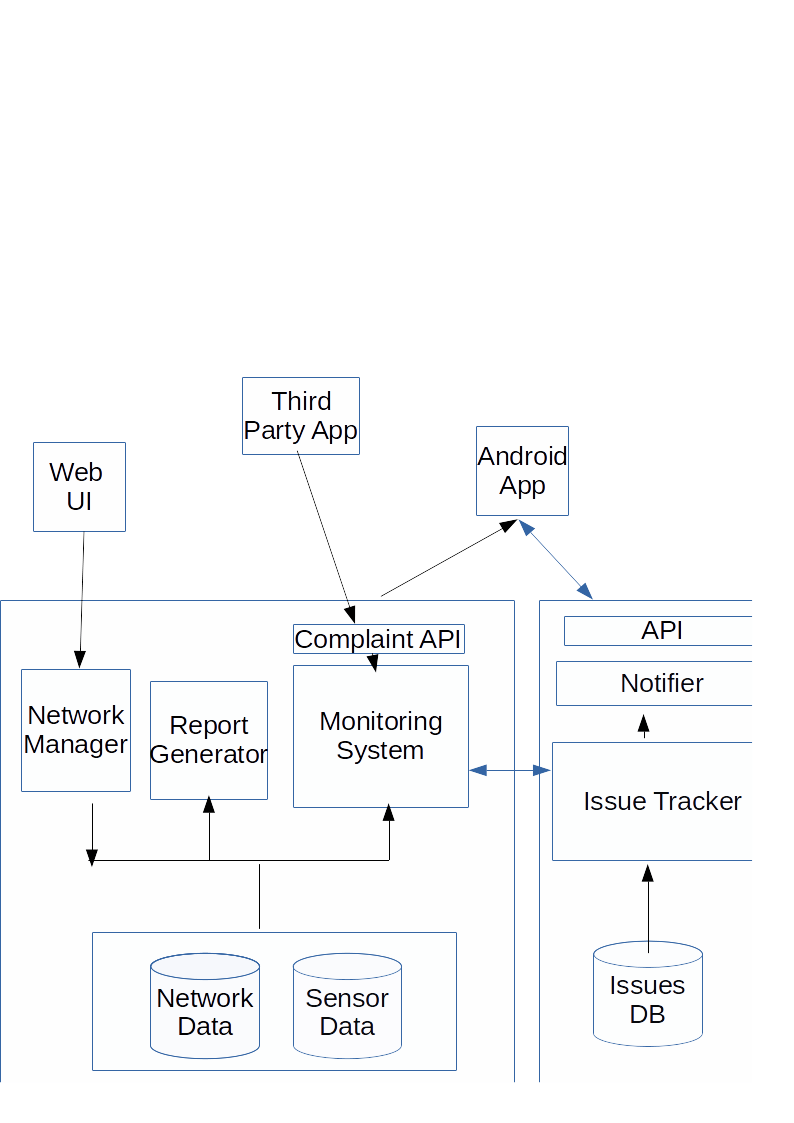
\includegraphics[scale=0.4]{HLD.png}
\subsection*{Monitoring System}
Scans the sensor data continuously for anomalies and reports the same to the issue tracker. Anomalies include breaches in threshold levels, leaks and external complaints. It also reports daily water requirements according to it's prediction.

\subsection*{Reports Generator}
Provides an API to get the following types of reports, each of which can be drilled down.
\begin{itemize}
\item Water consumption by aggregation.
\item Water consumption by time.
\item Water consumption by population.
\item Health of network assets.
\end{itemize}
\subsection*{Issue Tracker}
Keeps track of the status of resolution of issues. Also, notifies on creation of an issue to subscribers.
\subsection*{Network Manager}
Provides an API for creating the network and defining hierarchical aggregations.

\section*{Database Design}
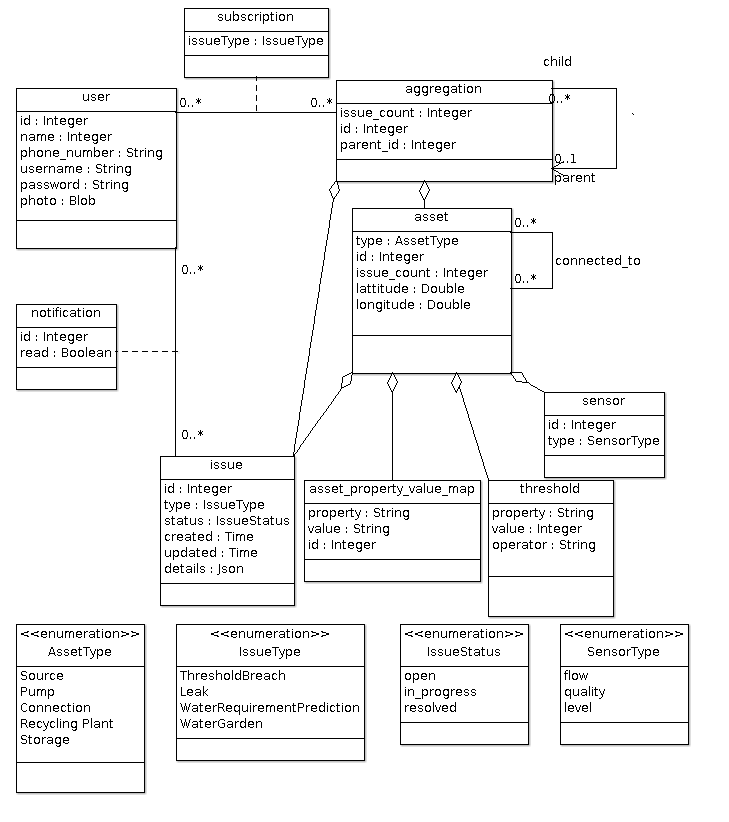
\includegraphics[scale=0.6]{DBDesign.png}

\section*{Low Level Design}
Following is the rough sketch of the main classes.\\\\
\begin{tabular}{|l|c|l|}
\hline
Class Name & Members & Methods\\
\hline
\hline
SensorMonitor & issueTracker & monitor(), predictWaterRequirement(), DetectLeaks()\\
\hline
ComplaintListener & issueTracker & getAggregations(), createComplaint()\\
\hline
IssueTracker & notifier & add(issue), resolve(issue)\\
\hline
Notifier & & notify()\\
\hline
ReportGenerator & & createAggregationBasedReport() \\&& createTimeBasedReport()\\&&createHealthBasedReport()\\
\hline
NetworkManager & & createNetwork(), createConnections()\\ &&modifyProperty(), createAggregation()\\
\hline 

\end{tabular}

\end{document}
